\documentclass[11pt,a4paper]{article}
\usepackage[T1]{fontenc}
\usepackage{graphicx}
\usepackage{isabelle,isabellesym}

% this should be the last package used
\usepackage{pdfsetup}

% urls in roman style, theory text in math-similar italics
\urlstyle{rm}
\isabellestyle{it}


\begin{document}

\title{Countable Ordinals}
\author{Brian Huffman}
\maketitle
\begin{abstract}
This development defines a well-ordered type of countable ordinals.
It includes notions of continuous and normal functions, recursively
defined functions over ordinals, least fixed-points, and derivatives.
Much of ordinal arithmetic is formalized, including exponentials and
logarithms. The development concludes with formalizations of Cantor
Normal Form and Veblen hierarchies over normal functions.
\end{abstract}

\tableofcontents

%\begin{center}
%  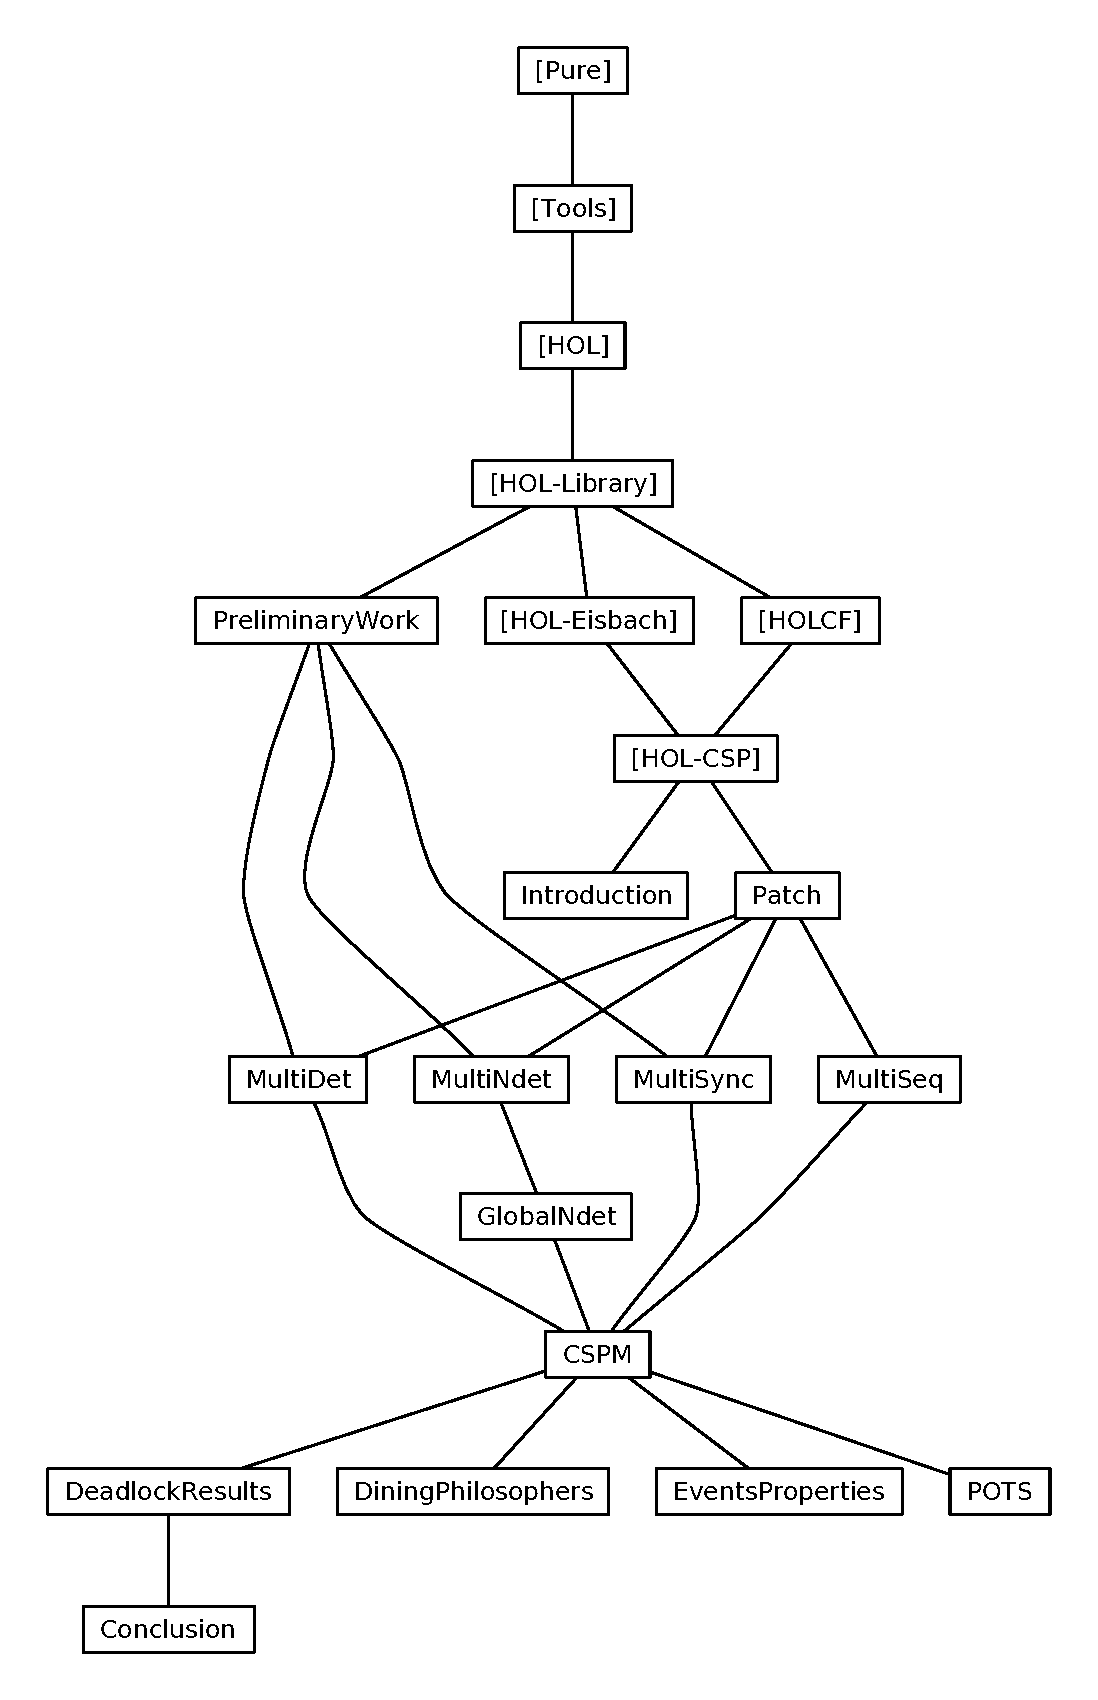
\includegraphics[scale=0.7]{session_graph}
%\end{center}

\newpage

\parindent 0pt\parskip 0.5ex

% generated text of all theories
\input{session}

\end{document}

%%% Local Variables:
%%% mode: latex
%%% TeX-master: t
%%% End:
